\subsection{LED-Streifen}\label{sec:LED}
Da die PVC-Platten sehr dunkel sind und nur durch die Tür Licht in die Kammer kommt, ist eine Beleuchtung notwendig. Dies wird mit einem einfachen LED-Streifen umgesetzt. Der gewählte LED-Streifen wird mit 24V versorgt und kann dank dem IC WS2811 mit dem Raspberry gesteuert werden. Es kann ein warmes oder kaltes Licht erzeugt werden. \\
\vspace{3mm}
Schaltplan:\\
\vspace{2mm}
\begin{figure}[H]
    \centering
    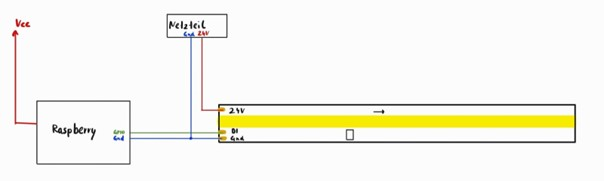
\includegraphics[scale=1]{image/schaltplanled.jpg}
    \caption{Schaltplan LED}
    \label{fig:enter-label}
\end{figure}
\vspace{3mm}
Der LED-Streifen wird mit demselben Netzteil als der Motor versorgt. Dieses liefert genau 24V. DI auf dem LED-Streifen steht für Daten In und wird über einen GPIO-Pin gesteuert. GND geht jeweils zum Raspberry Pi und zum Netzteil. \\
\vspace{3mm}
Damit auch die Ecken sauber an den Deckel der Kammer geklebt werden kann, wurde der LED-Streifen auseinandergeschnitten, um 90° gedreht und wieder mit Kabel verbunden. Da der UV-Strahler an dem Decker auf einem Aluprofil montiert ist, muss das Kabel über das Profil gehen, um eine durchgängige Verbindung zu erhalten. \\
\vspace{3mm}
Bei der Verdrahtung ist zu beachten, dass die Pfeile auf dem Streifen berücksichtig werden. 
 